\documentclass[border=6pt]{standalone}
% Shared preamble for web figures.  Each figure is a standalone .tex that
% \input's this file; scripts/make-figures.sh turns it into an SVG.
% Handouts pull the same file with \fig{Unit_X/<name>}.
\usepackage[T1]{fontenc}
\usepackage{helvet}
\renewcommand{\familydefault}{\sfdefault}
\renewcommand{\ttdefault}{pcr}  % Courier: a real Type 1 typewriter font
\usepackage{amsmath}
\usepackage{tikz}
\usetikzlibrary{arrows.meta,positioning,calc,shapes.symbols,shapes.geometric}

% Who makes the rules is the point of most diagrams in this book, so the
% colors mean the same thing everywhere: blue is a person, orange is the
% computer, green is an answer, pink is the human brain.
\definecolor{person}{HTML}{2C6FAE}
\definecolor{machine}{HTML}{D35400}
\definecolor{result}{HTML}{1E8449}
\definecolor{brainpink}{HTML}{C2185B}
\definecolor{ink}{HTML}{2C3E50}

\tikzset{
  doodle/.style={line width=1.5pt, line cap=round, line join=round, draw=ink},
  box/.style={draw, rounded corners=5pt, line width=1.1pt, align=center,
              inner sep=7pt, minimum height=1.0cm, font=\small},
  personbox/.style={box, draw=person, fill=person!10},
  machinebox/.style={box, draw=machine, fill=machine!10},
  resultbox/.style={box, draw=result, fill=result!10},
  plainbox/.style={box, draw=ink!70, fill=ink!4},
  flow/.style={-{Stealth[length=8pt]}, line width=1.4pt, draw=ink},
}

% A person (blue) and a robot head (orange) as small icons.
% \personicon{x}{y}{scale}   \roboticon{x}{y}{scale}
\newcommand{\personicon}[3]{%
  \begin{scope}[shift={(#1,#2)}, scale=#3]
    \fill[person] (0,0.62) circle (0.28);
    \fill[person, rounded corners=6pt] (-0.42,-0.55) rectangle (0.42,0.28);
  \end{scope}}
\newcommand{\roboticon}[3]{%
  \begin{scope}[shift={(#1,#2)}, scale=#3]
    \draw[machine, line width=1.2pt] (0,0.5) -- (0,0.72);
    \fill[machine] (0,0.78) circle (0.08);
    \draw[machine, line width=1.4pt, fill=machine!12, rounded corners=4pt] (-0.5,-0.45) rectangle (0.5,0.5);
    \fill[ink] (-0.2,0.12) circle (0.08);
    \fill[ink] (0.2,0.12) circle (0.08);
    \draw[ink, line width=1pt] (-0.22,-0.22) -- (0.22,-0.22);
  \end{scope}}

\begin{document}
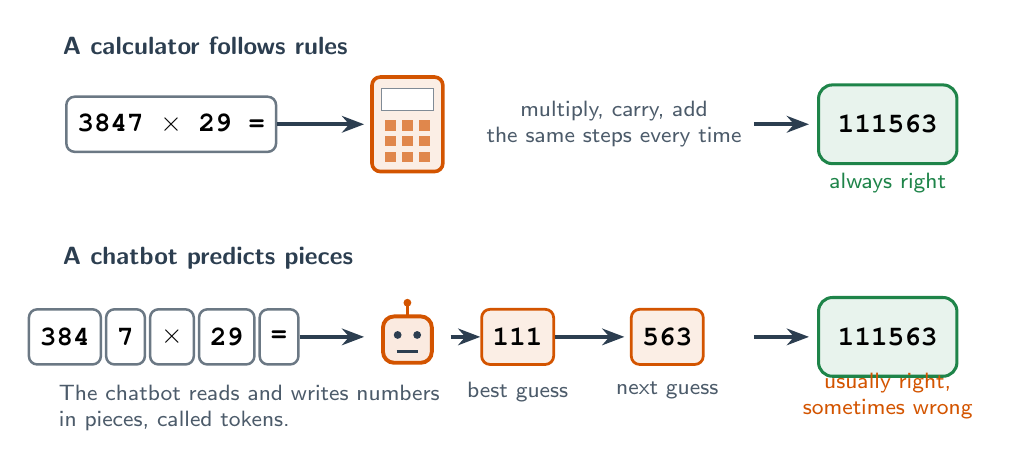
\begin{tikzpicture}[
  tok/.style={draw=ink!70, fill=white, rounded corners=3pt, line width=0.9pt, font=\ttfamily\bfseries, minimum height=0.7cm, inner sep=4pt},
  guess/.style={draw=machine, fill=machine!10, rounded corners=3pt, line width=1pt, font=\ttfamily\bfseries, minimum height=0.7cm, inner sep=4pt},
  head/.style={font=\small\bfseries, text=ink, anchor=west},
  note/.style={font=\footnotesize, text=ink!85, align=center},
]
% Top: a calculator follows the rules of multiplication.
\node[head] at (-0.2,1.0) {A calculator follows rules};
\node[tok] (q1) at (1.3,0) {3847 $\times$ 29 =};
% calculator icon
\begin{scope}[shift={(4.3,0)}]
  \draw[machine, line width=1.3pt, fill=machine!10, rounded corners=3pt] (-0.45,-0.6) rectangle (0.45,0.6);
  \fill[white] (-0.33,0.18) rectangle (0.33,0.45); \draw[ink!60] (-0.33,0.18) rectangle (0.33,0.45);
  \foreach \i in {-1,0,1} \foreach \j in {0,1,2} \fill[machine!70] (\i*0.22-0.07,-0.48+\j*0.2) rectangle ++(0.14,0.13);
\end{scope}
\draw[flow] (q1.east) -- (3.75,0);
\node[note, anchor=west, text width=3.6cm] (w) at (5.0,0) {multiply, carry, add\\the same steps every time};
\draw[flow] (8.7,0) -- (9.4,0);
\node[resultbox, font=\ttfamily\bfseries] at (10.4,0) {111563};
\node[note, text=result] at (10.4,-0.75) {always right};

% Bottom: a chatbot predicts the answer one piece at a time.
\node[head] at (-0.2,-1.7) {A chatbot predicts pieces};
\node[tok] (a) at (-0.05,-2.7) {384};
\node[tok, right=1pt of a] (b) {7};
\node[tok, right=1pt of b] (c) {$\times$};
\node[tok, right=1pt of c] (d) {29};
\node[tok, right=1pt of d] (e) {=};
\roboticon{4.3}{-2.75}{0.62}
\draw[flow] (e.east) -- (3.75,-2.7);
\node[guess] (g1) at (5.7,-2.7) {111};
\node[note, anchor=north] at (5.7,-3.15) {best guess};
\node[guess] (g2) at (7.6,-2.7) {563};
\node[note, anchor=north] at (7.6,-3.15) {next guess};
\draw[flow] (4.85,-2.7) -- (g1.west);
\draw[flow, shorten >=2pt] (g1.east) -- (g2.west);
\draw[flow] (8.7,-2.7) -- (9.4,-2.7);
\node[resultbox, font=\ttfamily\bfseries] at (10.4,-2.7) {111563};
\node[note, text=machine] at (10.4,-3.45) {usually right,\\sometimes wrong};
\node[note, anchor=west, text width=5cm, align=left] at (-0.25,-3.6) {The chatbot reads and writes numbers in pieces, called tokens.};
\end{tikzpicture}
\end{document}
